% FSB Presentation — Seminar: ISO 26262 i ISO 21448 (SOTIF)
% Standalone: does not touch docs/main.tex. Build with Tectonic.
%
% Two builds from this one file:
%   presentation.tex        -> slides only
%   presentation-notes.tex  -> slides + speaker notes (defines \NOTESONLY)
%
% Diagrams use plain rounded nodes, not tikz's `mindmap` library: mindmap's
% circular concepts overlap at this text length and its font handling mangled
% digits ("21448" rendered as "2144o").

\documentclass{beamer}

\usepackage{iftex}
\ifPDFTeX
  \usepackage{cmap}
  \usepackage[utf8]{inputenc}
  \usepackage[T1]{fontenc}
  \usepackage{lmodern}
\fi
\usepackage[croatian]{babel}

% Speaker notes: shown only in the -notes build.
\ifdefined\NOTESONLY
  \setbeameroption{show notes}
\fi

\usepackage{tikz}
\usetikzlibrary{positioning}

\usetheme{Madrid}
\usecolortheme{whale}
\setbeamertemplate{navigation symbols}{}

\definecolor{fusa}{RGB}{31,90,140}
\definecolor{sotif}{RGB}{176,88,20}
\definecolor{rootgray}{RGB}{62,62,72}

% --- One visual language for every diagram ---
\tikzset{
  mroot/.style   = {rounded corners=7pt, fill=rootgray, text=white, align=center,
                    font=\small\bfseries, minimum width=2.7cm,
                    minimum height=1.15cm, inner sep=4pt},
  mfusa/.style   = {mroot, fill=fusa},
  msotif/.style  = {mroot, fill=sotif},
  % Leaves: fixed text width so long labels wrap instead of stretching the box.
  mleaf/.style     = {mroot, minimum width=2.8cm, minimum height=1.05cm,
                      text width=2.5cm, font=\scriptsize\bfseries},
  leaffusa/.style  = {mleaf, fill=fusa!72},
  leafsotif/.style = {mleaf, fill=sotif!72},
  leafn/.style     = {mleaf, fill=rootgray!62},   % neutral: belongs to neither norm
  link/.style    = {draw=black!40, line width=1.1pt},
}

\title[ISO 26262 i ISO 21448]{Uloga normi ISO 26262 i ISO 21448 (SOTIF) u osiguravanju sigurnosti sustava automatizirane vožnje}
\author{Ivan Noršić}
\institute[FSB]{Fakultet strojarstva i brodogradnje\\Sveučilište u Zagrebu}
\date{Zagreb, 2026.}

\begin{document}

% ============================================================
\begin{frame}
  \titlepage
\end{frame}

\note{
Dobar dan. Tema mog seminara je uloga dviju normi --- ISO 26262 i ISO 21448,
poznatije kao SOTIF --- u osiguravanju sigurnosti sustava automatizirane vožnje.

Cilj izlaganja: pokazati da te dvije norme NISU konkurentske, nego pokrivaju
dvije različite vrste sigurnosnog rizika, i da su tek zajedno potpune.

Plan: prvo zašto uopće trebamo dvije norme, zatim svaka posebno, pa usporedba,
izazovi integracije i zaključak. Ima devet slajdova, traje oko deset minuta.
}

% ============================================================
\begin{frame}{Zašto dvije norme?}
  \begin{center}
  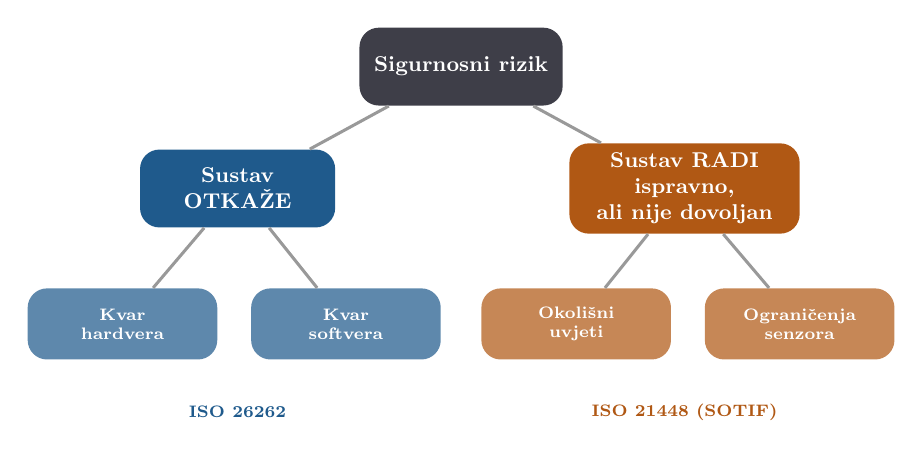
\begin{tikzpicture}[scale=0.86, transform shape]

    \node[mroot, minimum width=3.0cm] (r) at (0, 2.7) {Sigurnosni rizik};

    \node[mfusa,  text width=2.6cm] (l) at (-3.3, 0.9) {Sustav\\OTKAŽE};
    \node[msotif, text width=3.0cm, minimum width=3.4cm] (d) at (3.3, 0.9)
      {Sustav RADI ispravno,\\ali nije dovoljan};

    \node[leaffusa]  (l1) at (-5.0, -1.1) {Kvar\\hardvera};
    \node[leaffusa]  (l2) at (-1.7, -1.1) {Kvar\\softvera};
    \node[leafsotif] (d1) at (1.7, -1.1)  {Okolišni\\uvjeti};
    \node[leafsotif] (d2) at (5.0, -1.1)  {Ograničenja\\senzora};

    \draw[link] (r) -- (l);
    \draw[link] (r) -- (d);
    \draw[link] (l) -- (l1);
    \draw[link] (l) -- (l2);
    \draw[link] (d) -- (d1);
    \draw[link] (d) -- (d2);

    \node[font=\scriptsize\bfseries, text=fusa]  at (-3.3, -2.4) {ISO 26262};
    \node[font=\scriptsize\bfseries, text=sotif] at (3.3, -2.4)  {ISO 21448 (SOTIF)};
  \end{tikzpicture}
  \end{center}
\end{frame}

\note{
Ovo je ključna slika cijelog izlaganja. Sve ostalo je razrada.

Sigurnosni rizik u vozilu dolazi iz dva potpuno različita izvora.

Prvi: sustav OTKAŽE. Nešto se pokvari --- pukne senzor, zablokira se procesor,
softver ima grešku. Sustav je dobro projektiran, ali ne radi kako treba.
Time se bavi ISO 26262, funkcijska sigurnost.

Drugi, i to je manje očit: sustav RADI potpuno ispravno, ništa nije pokvareno,
svaka komponenta radi točno ono za što je projektirana --- a ishod je svejedno
opasan. Zašto? Jer sam dizajn nije dovoljan za sve uvjete. Magla, zasljepljujuće
sunce, ograničena rezolucija senzora. To se zove funkcionalna insuficijencija i
time se bavi ISO 21448, odnosno SOTIF.

Naglasiti razliku jednom rečenicom: ISO 26262 pretpostavlja da je sustav dobro
dizajniran ali može otkazati; SOTIF pretpostavlja da sustav radi ispravno ali
mu dizajn može biti nedovoljan.

Ako publika zapamti samo ovaj slajd, izlaganje je uspjelo.
}

% ============================================================
\begin{frame}{ISO 26262 --- funkcijska sigurnost}
  \begin{center}
  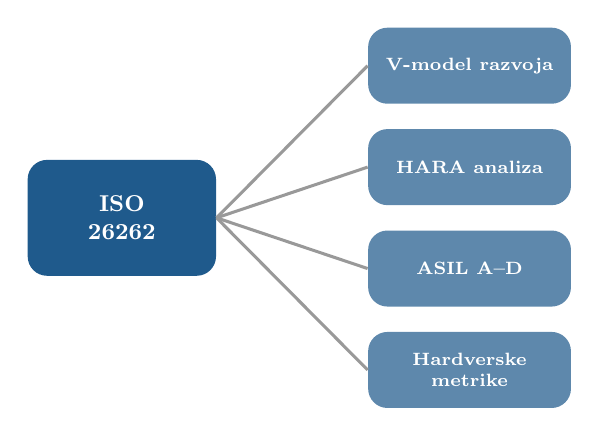
\begin{tikzpicture}[scale=0.92, transform shape]

    \node[mfusa, minimum width=2.6cm, minimum height=1.6cm,
          font=\small\bfseries] (r) at (-3.4, 0) {ISO\\26262};

    \node[leaffusa] (a) at (1.4, 2.1)  {V-model razvoja};
    \node[leaffusa] (b) at (1.4, 0.7)  {HARA analiza};
    \node[leaffusa] (c) at (1.4, -0.7) {ASIL A--D};
    \node[leaffusa] (d) at (1.4, -2.1) {Hardverske metrike};

    \draw[link] (r.east) -- (a.west);
    \draw[link] (r.east) -- (b.west);
    \draw[link] (r.east) -- (c.west);
    \draw[link] (r.east) -- (d.west);
  \end{tikzpicture}
  \end{center}

  \begin{center}
    \small Cilj: \textbf{odsutnost rizika od kvarova E/E sustava}
  \end{center}
\end{frame}

\note{
ISO 26262 je zrela, dobro uspostavljena norma. Bavi se elektroničkim i
električnim sustavima u vozilu --- kraticom E/E.

Četiri stupa:

V-model --- razvojni proces. Lijeva grana silazi od zahtjeva prema
implementaciji, desna se penje kroz verifikaciju i validaciju. Linearan,
strukturiran. Zapamtite riječ ,,linearan'' --- vratit ćemo joj se kod integracije.

HARA --- analiza opasnosti i procjena rizika. Provodi se u fazi koncepta i iz
nje izlaze sigurnosni ciljevi. Detaljnije na sljedećem slajdu.

ASIL --- klasifikacija strogosti sigurnosnih zahtjeva, od A do D.

Hardverske metrike --- kvantitativni ciljevi za slučajne kvarove hardvera.
Ako netko pita: SPFM, LFM i PMHF; postaju stroži kako raste ASIL razina.

Ključna rečenica: cilj je odsutnost neprihvatljivog rizika koji proizlazi iz
KVARA elektroničkog sustava.
}

% ============================================================
\begin{frame}{Od rizika do ASIL razine}
  \begin{center}
  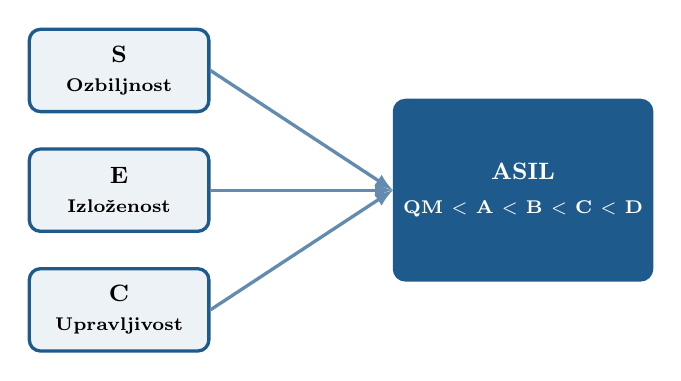
\begin{tikzpicture}[scale=0.95, transform shape,
      box/.style={draw=fusa, very thick, rounded corners, fill=fusa!8,
                  minimum width=2.4cm, minimum height=1.1cm, align=center,
                  font=\small\bfseries},
      arr/.style={-latex, very thick, draw=fusa!70}]

    \node[box] (s) at (-2.6, 1.6)  {S\\\scriptsize Ozbiljnost};
    \node[box] (e) at (-2.6, 0)    {E\\\scriptsize Izloženost};
    \node[box] (c) at (-2.6, -1.6) {C\\\scriptsize Upravljivost};

    \node[box, fill=fusa, text=white, minimum width=3.2cm, minimum height=2.4cm]
      (asil) at (2.8, 0) {ASIL\\[2pt]\scriptsize QM $<$ A $<$ B $<$ C $<$ D};

    \draw[arr] (s.east) -- (asil.west);
    \draw[arr] (e.east) -- (asil.west);
    \draw[arr] (c.east) -- (asil.west);
  \end{tikzpicture}
  \end{center}

  \begin{center}
    \small Viša razina $\Rightarrow$ stroži zahtjevi razvoja, testiranja i dokumentacije
  \end{center}
\end{frame}

\note{
Kako se dolazi do ASIL razine? Kombinacijom triju parametara.

S --- ozbiljnost moguće štete, od S0 do S3.
E --- izloženost, koliko se često vozilo nađe u toj situaciji, od E0 do E4.
C --- upravljivost, može li vozač ili drugi sudionik izbjeći štetu, od C0 do C3.

Njihova kombinacija daje ASIL razinu. QM znači ,,samo upravljanje kvalitetom'',
nisu potrebne posebne sigurnosne mjere. Zatim A, B, C, i D kao najstroža.

Primjer za intuiciju: električni podizač prozora je QM ili ASIL A. Sustav
autonomnog kočenja je ASIL D --- najozbiljnije posljedice kvara.

Što znači viša razina u praksi? Za ASIL D traži se formalna verifikacija
softvera, redundancija hardvera i neovisna procjena sigurnosti.

Ako pitaju za dekompoziciju: zahtjev visoke razine smije se raspodijeliti na
više neovisnih elemenata niže razine, ako se dokaže njihova neovisnost.
}

% ============================================================
\begin{frame}{ISO 21448 --- SOTIF}
  \begin{center}
  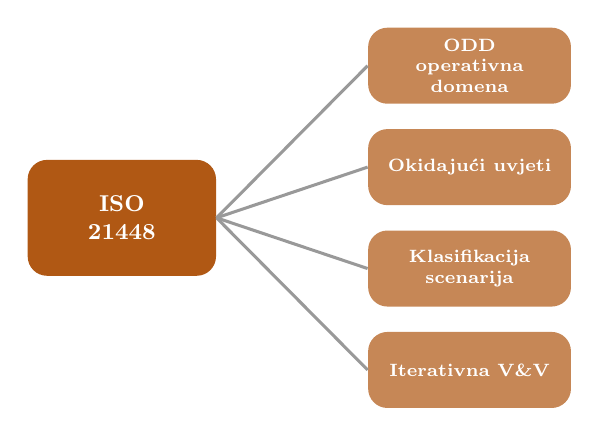
\begin{tikzpicture}[scale=0.92, transform shape]

    \node[msotif, minimum width=2.6cm, minimum height=1.6cm,
          font=\small\bfseries] (r) at (-3.4, 0) {ISO\\21448};

    \node[leafsotif] (a) at (1.4, 2.1)  {ODD\\operativna domena};
    \node[leafsotif] (b) at (1.4, 0.7)  {Okidajući uvjeti};
    \node[leafsotif] (c) at (1.4, -0.7) {Klasifikacija scenarija};
    \node[leafsotif] (d) at (1.4, -2.1) {Iterativna V\&V};

    \draw[link] (r.east) -- (a.west);
    \draw[link] (r.east) -- (b.west);
    \draw[link] (r.east) -- (c.west);
    \draw[link] (r.east) -- (d.west);
  \end{tikzpicture}
  \end{center}

  \begin{center}
    \small Cilj: \textbf{odsutnost rizika od ograničenja performansi}
  \end{center}
\end{frame}

\note{
SOTIF --- Safety Of The Intended Functionality, sigurnost namijenjene
funkcionalnosti. Ovdje nema kvara. Sve radi po specifikaciji.

Četiri stupa:

ODD, operativna domena --- skup uvjeta pod kojima je sustav projektiran raditi
sigurno: tipovi cesta, raspon brzina, vremenski i svjetlosni uvjeti. Izlazak iz
ODD-a, ili rad na njegovom rubu, tipičan je izvor SOTIF rizika.

Okidajući uvjeti --- okolnosti koje navedu ispravan sustav da proizvede opasan
ishod. Tri vrste: okolišni (magla, kiša, refleksije), scenarijski (neočekivano
ponašanje drugih sudionika) i tehnološki (rezolucija senzora, blato na kameri).

Klasifikacija scenarija --- sljedeći slajd.

Iterativna verifikacija i validacija. Ovdje NEMA V-modela. Proces je ciklički:
analiziraj, izmijeni, testiraj, pa ispočetka. To je druga riječ koju treba
zapamtiti za slajd o integraciji.
}

% ============================================================
\begin{frame}{Četiri područja scenarija}
  \vspace{0.2cm}
  \begin{center}
  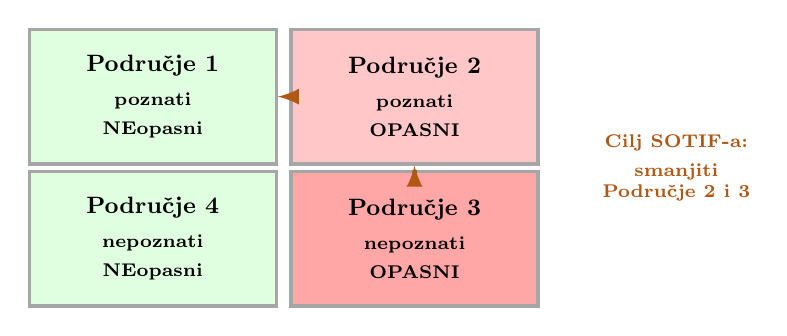
\begin{tikzpicture}[scale=0.95, transform shape,
      cell/.style={draw=black!35, very thick, minimum width=3.3cm,
                   minimum height=1.8cm, align=center, font=\small\bfseries}]

    \node[cell, fill=green!12] (p1) at (-2.4, 1.0)  {Područje 1\\[2pt]\scriptsize poznati\\\scriptsize NEopasni};
    \node[cell, fill=red!22]   (p2) at (1.1, 1.0)   {Područje 2\\[2pt]\scriptsize poznati\\\scriptsize OPASNI};
    \node[cell, fill=green!12] (p4) at (-2.4, -0.9) {Područje 4\\[2pt]\scriptsize nepoznati\\\scriptsize NEopasni};
    \node[cell, fill=red!35]   (p3) at (1.1, -0.9)  {Područje 3\\[2pt]\scriptsize nepoznati\\\scriptsize OPASNI};

    \draw[-latex, ultra thick, draw=sotif] (p3) -- (p2);
    \draw[-latex, ultra thick, draw=sotif] (p2) -- (p1);

    \node[align=center, font=\scriptsize\bfseries, text=sotif] at (4.6, 0.05)
      {Cilj SOTIF-a:\\[3pt] smanjiti\\Područje 2 i 3};
  \end{tikzpicture}
  \end{center}
\end{frame}

\note{
Dvije osi: je li scenarij poznat, i je li opasan. Iz toga četiri područja.

Područje 1: poznati i neopasni. Tu želimo biti.
Područje 4: nepoznati, ali neopasni. Ne smetaju nam.

Zanimljiva su druga dva.

Područje 2: poznati OPASNI scenariji. Znamo za njih. Rješenje: mjere koje ih
prebacuju u sigurno područje --- poboljšanje senzora, redundancija, fail-safe
mehanizmi poput nužnog kočenja.

Područje 3: nepoznati opasni scenariji. Najteža kategorija --- ne znamo ni da
postoje. Jedini put je sustavno testiranje i analiza, kojima ih prevodimo u
poznate, dakle u Područje 2, a onda ih rješavamo.

Pokazati strelice: cilj je gurati scenarije prema gore i lijevo, iz 3 u 2, pa
iz 2 u 1.

To je bit SOTIF procesa: sustavno smanjivanje prostora nepoznatih opasnih
scenarija. Nikad ne dođe do nule --- ostaje rezidualni rizik.
}

% ============================================================
\begin{frame}{Usporedba: dvije strane iste medalje}
  \begin{center}
  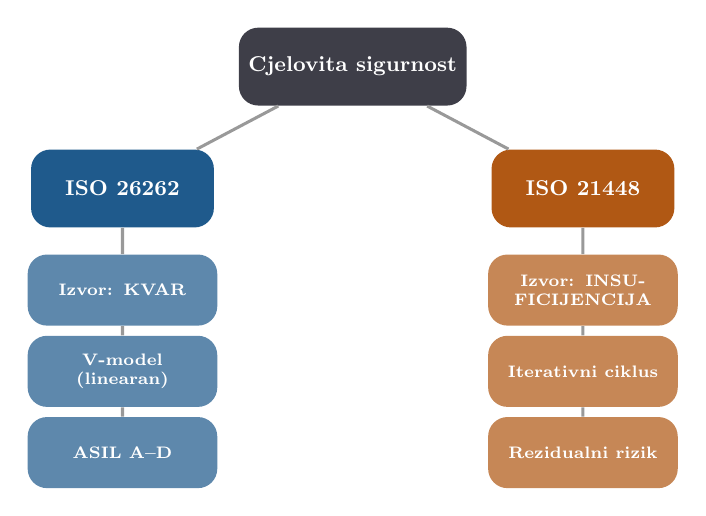
\begin{tikzpicture}[scale=0.86, transform shape]

    \node[mroot, minimum width=3.2cm] (r) at (0, 2.8) {Cjelovita sigurnost};

    \node[mfusa]  (f) at (-3.4, 1.0) {ISO 26262};
    \node[msotif] (s) at (3.4, 1.0)  {ISO 21448};

    \node[leaffusa] (f1) at (-3.4, -0.5) {Izvor: KVAR};
    \node[leaffusa] (f2) at (-3.4, -1.7) {V-model (linearan)};
    \node[leaffusa] (f3) at (-3.4, -2.9) {ASIL A--D};

    \node[leafsotif] (s1) at (3.4, -0.5) {Izvor: INSUFICIJENCIJA};
    \node[leafsotif] (s2) at (3.4, -1.7) {Iterativni ciklus};
    \node[leafsotif] (s3) at (3.4, -2.9) {Rezidualni rizik};

    \draw[link] (r) -- (f);
    \draw[link] (r) -- (s);
    \draw[link] (f) -- (f1);
    \draw[link] (f1) -- (f2);
    \draw[link] (f2) -- (f3);
    \draw[link] (s) -- (s1);
    \draw[link] (s1) -- (s2);
    \draw[link] (s2) -- (s3);
  \end{tikzpicture}
  \end{center}
\end{frame}

\note{
Sad spajamo. Ovo je usporedni pregled.

Lijevo ISO 26262: izvor opasnosti je KVAR, razvojni model je V-model, rizik se
klasificira ASIL razinama.

Desno ISO 21448: izvor opasnosti je funkcionalna INSUFICIJENCIJA, model je
iterativan, a rizik se izražava kao rezidualni rizik --- bez ASIL ljestvice.

Ključna poanta, i to naglasiti: ovo nisu suparničke norme i ne biramo jednu.
SOTIF sam po sebi NIJE potpun pristup --- mora se koristiti zajedno s
funkcijskom sigurnošću. Isto vrijedi obrnuto: ISO 26262 ne pokriva rizike
nedeterminističkih algoritama, uključujući strojno učenje.

Za potpuno sigurnosno osiguranje automatiziranog vozila obje se norme moraju
primjenjivati istodobno. Otud i naslov slajda --- dvije strane iste medalje.
}

% ============================================================
\begin{frame}{Izazovi integracije}
  \begin{center}
  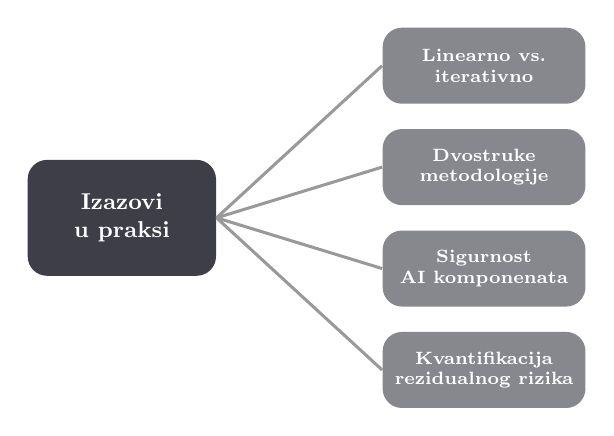
\begin{tikzpicture}[scale=0.92, transform shape]

    \node[mroot, minimum width=2.6cm, minimum height=1.6cm,
          font=\small\bfseries] (r) at (-3.4, 0) {Izazovi\\u praksi};

    \node[leafn] (a) at (1.6, 2.1)  {Linearno vs.\\iterativno};
    \node[leafn] (b) at (1.6, 0.7)  {Dvostruke\\metodologije};
    \node[leafn] (c) at (1.6, -0.7) {Sigurnost\\AI komponenata};
    \node[leafn] (d) at (1.6, -2.1) {Kvantifikacija\\rezidualnog rizika};

    \draw[link] (r.east) -- (a.west);
    \draw[link] (r.east) -- (b.west);
    \draw[link] (r.east) -- (c.west);
    \draw[link] (r.east) -- (d.west);
  \end{tikzpicture}
  \end{center}
\end{frame}

\note{
Komplementarnost je jasna u teoriji. U praksi integracija nosi četiri izazova.

Prvi: nepodudarnost razvojnih modela. V-model je linearan, SOTIF je iterativan.
Ne postoji jednostavno preslikavanje aktivnosti jedne norme na drugu.

Drugi: vođenje dvaju paralelnih sigurnosnih procesa. Povećava složenost, traži
opsežnu dokumentaciju i rigorozno upravljanje životnim ciklusom.

Treći: sigurnost AI komponenata. Sustavi sa strojnim učenjem teško se uklapaju
u tradicionalni, deterministički okvir ISO 26262. To je i motiviralo prilagodbu
procesnih zahtjeva norme.

Četvrti, i po mom mišljenju najozbiljniji: kvantifikacija rezidualnog rizika.
ISO 26262 ima jasno definirane ASIL razine. SOTIF nema konsenzus oko toga koji
je prag rezidualnog rizika prihvatljiv. To je otvoreno pitanje struke.

Literatura ipak pokazuje da je holistički pristup ostvariv --- zajednička
definicija sustava, integrirano testiranje i kontinuirana validacija kroz
cijeli životni ciklus.
}

% ============================================================
\begin{frame}{Zaključak}
  \vspace{0.3cm}
  \begin{itemize}
    \setlength{\itemsep}{0.7em}
    \item \textcolor{fusa}{\textbf{ISO 26262}} pokriva rizik od \textbf{kvara} E/E sustava.
    \item \textcolor{sotif}{\textbf{ISO 21448}} pokriva rizik od \textbf{nedostatnosti} ispravnog sustava.
    \item Norme su \textbf{komplementarne} --- nijedna sama nije dovoljna.
    \item Integracija je ostvariva, ali otvoreni izazovi ostaju.
  \end{itemize}

  \vspace{0.5cm}
  \begin{center}
    \footnotesize\itshape
    Postoje i druge norme relevantne za sigurnost automatizirane vožnje;\\
    ovaj se rad na njih ne fokusira.
  \end{center}

  \vspace{0.4cm}
  \begin{center}
    \large\bfseries Hvala na pažnji.
  \end{center}
\end{frame}

\note{
Sažetak u tri rečenice.

ISO 26262 pokriva rizik koji dolazi od kvara elektroničkog sustava.
ISO 21448 pokriva rizik koji dolazi od toga da ispravan sustav nije dovoljan
za sve uvjete.
Komplementarne su --- nijedna sama ne daje potpunu sliku sigurnosti.

Integracija je ostvariva, što pokazuje pregledana literatura, ali ostaju
otvoreni izazovi --- prije svega prag prihvatljivog rezidualnog rizika.

Zadnja rečenica na slajdu: postoje i druge norme u ovom području. Namjerno ih
ne otvaram --- opseg seminara su ove dvije. Ako netko pita, reći ću samo da
šire područje pokriva scenarijsku evaluaciju i sigurnosni slučaj, i ponuditi
da o tome porazgovaramo izvan izlaganja.

Hvala na pažnji. Otvoren sam za pitanja.
}

\end{document}
